%%%%%%%%%%%%%%%%%%%%%%% file template.tex %%%%%%%%%%%%%%%%%%%%%%%%%
%
% This is a general template file for the LaTeX package SVJour3
% for Springer journals.          Springer Heidelberg 2010/09/16
%
% Copy it to a new file with a new name and use it as the basis
% for your article. Delete % signs as needed.
%
% This template includes a few options for different layouts and
% content for various journals. Please consult a previous issue of
% your journal as needed.
%
%%%%%%%%%%%%%%%%%%%%%%%%%%%%%%%%%%%%%%%%%%%%%%%%%%%%%%%%%%%%%%%%%%%
%
% First comes an example EPS file -- just ignore it and
% proceed on the \documentclass line
% your LaTeX will extract the file if required
\begin{filecontents*}{example.eps}
%!PS-Adobe-3.0 EPSF-3.0
%%BoundingBox: 19 19 221 221
%%CreationDate: Mon Sep 29 1997
%%Creator: programmed by hand (JK)
%%EndComments
gsave
newpath
  20 20 moveto
  20 220 lineto
  220 220 lineto
  220 20 lineto
closepath
2 setlinewidth
gsave
  .4 setgray fill
grestore
stroke
grestore
\end{filecontents*}
%
\RequirePackage{fix-cm}
%
%\documentclass{svjour3}                     % onecolumn (standard format)
%\documentclass[smallcondensed]{svjour3}     % onecolumn (ditto)
\documentclass[smallextended]{svjour3}       % onecolumn (second format)
%\documentclass[twocolumn]{svjour3}          % twocolumn
%
\smartqed  % flush right qed marks, e.g. at end of proof
%
\usepackage{graphicx}
%
% \usepackage{mathptmx}      % use Times fonts if available on your TeX system
%
% insert here the call for the packages your document requires
%\usepackage{latexsym}
\usepackage{natbib}
% etc.
%
% please place your own definitions here and don't use \def but
% \newcommand{}{}
%
% Insert the name of "your journal" with
% \journalname{myjournal}
%

\usepackage{amsmath}    

\begin{document}

\title{Excess thermodynamic and elastic properties of mineral and melt solutions: modelling and implications for phase relations and seismic velocities}
%\subtitle{Do you have a subtitle?\\ If so, write it here}

\titlerunning{Excess properties of mineral and melt solutions}        % if too long for running head

\author{R. Myhill}

%\authorrunning{Short form of author list} % if too long for running head

\institute{R. Myhill \at
              Bayerisches Geoinstitut, Universit\"{a}t Bayreuth, Universit\"{a}tsstrasse 30, 95447 Bayreuth, Germany\\
              \email{myhill.bob@gmail.com}}

\date{Received: date / Accepted: date}
% The correct dates will be entered by the editor


\maketitle

\begin{abstract}


This paper describes an extension to the subregular Margules mixing model which employs intermediate compounds to define the excess thermodynamic properties of solid solutions. Mathematical derivations are provided for excess thermodynamic properties (enthalpy, entropy, volume) and their pressure and temperature derivatives (bulk modulus, thermal expansion etc.). Heuristics are suggested for intermediate compounds where individual thermodynamic properties are poorly constrained.

Examples of pyroxene, garnet and melt solutions are presented, which show that accurate modelling of phase relations and seismic velocities requires absolute excess volumes to decrease as a function of pressure. The formulation proposed here allows for a wealth of experimental data to be incorporated into solution models, and is expected to be important for geochemical and geophysical models of the Earth and other planetary bodies.

\keywords{high pressure \and excess properties \and solution model \and solid \and melt \and elasticity}
\end{abstract}



\section{Introduction}
Thermodynamic models of solid and liquid solutions are increasingly used to calculate phase relations and seismic properties over large pressure and temperature ranges. Research into mantle phase relations, subduction and differentiation of the early Earth frequently involves calculations spanning thousands of Kelvin and tens of gigapascals. Over such huge ranges, excess entropy and volume are unlikely to remain constant with respect to pressure and temperature. For example, absolute excess volumes usually decrease with increasing pressure. The implication is that to provide a good estimate of phase relations and seismic velocities, solution models must be flexible enough to accommodate changes in elastic and thermodynamic derivatives, such as the bulk modulus.

The majority of solution models take a form where excess Gibbs free energies (relative to ideal solutions) are either constant as a function of temperature and pressure, or are linear, such that interaction energies between phases $i$ and $j$ take the form
\begin{equation}
  W_{ij}^{\mathcal{G}} = W_{ij}^{\mathcal{E}} + W_{ij}^{\mathcal{V}}P - W_{ij}^{\mathcal{S}}T
  \label{eqn:trad_form}
\end{equation}
The entropic $\mathcal{S}$ and volumetric $\mathcal{V}$ terms are assumed to remain constant with temperature and pressure. Indeed, in the absence of calorimetric data, it is often assumed that $W_{ij}^{\mathcal{S}} = 0$. Over small pressure and temperature ranges, a linear approximation is usually satisfactory for free energy calculations (for example, to calculate the width of a solvus or equilibrium with other phases). However, thermodynamic models are now being extended over much larger pressure and temperature ranges \citep{SLB2011, HP2011, HHPH2013, DKS2013}, where such approximations may not be satisfactory.

Thermoelastic models are also increasingly being used to interpret seismic data in terms of the temperature and composition of the deep Earth. Studies have focussed on Earth's mantle \citep[e.g.][]{DGDSBR2012, MCDRT2012, DCT2012} and core \citep[e.g.][]{SGGFMM2000,SFGMM2004}, and with the successful deployment of seismometers may soon extend to Mars \citep{GLZR2014}. Again, the bulk modulus imposed by the constant excess volume approximation may be a significant and unnecessary contributor to error in these studies, especially for metallic liquids, where excess volumes at low pressures are often very large. 

This paper first discusses some observations of excess properties in solid solutions, and the physical origins of these causes. Useful rules-of-thumb are provided to provide the reader with predictions of excess propetries were only limited information is available. An adaptation of the subregular Margules mixing model is then presented, using intermediate compounds to describe the excess properties of the solid solution. This formulation is used to model the thermodynamics of three solid solutions from the literature. 


\section{Observations and models of excess properties} 
\subsection{Excess thermoelastic and thermodynamic properties and their causes}
\label{sec:obs}
Chemical compounds which form solutions by exchanging ions with similar radii, charge and field strength typically exhibit near-ideal mixing; that is, their thermodynamic properties can be described as a mechanical mixture with an additional entropy attributable to the various potential configurations of the enxchanged ions. In the geological sciences, Fe$^{2+}$-Mg$^{2+}$ exchange is a good example of near-ideal mixing in several minerals. For example, the almandine-pyrope solid solution exhibits negligible excess volumes and entropies and excess energies of only a few kilojoules per mole \citep[on a three-site basis;][]{GCT1996, WPHJG2014}. In contrast, exchange involving very different species is commonly associated with large excess properties. For example, the exchange of Mg$^{2+}$ for the much larger cation Ca$^{2+}$ \citep[0.89 \AA and 1.12 \AA respectively;][]{Shannon1976}) in the pyrope-grossular solid solution leads to excess energies of $\sim$30 kJ/mol \citep{GCT1996}. 

Where the exchanging species are of different sizes but interact weakly with each other, excess volumes tend to be positive. This is true of both liquids \citep[e.g. benzene-cyclohexane;][]{FM1965} and solids \citep[e.g. pyrope-grossular;][]{GCT1996}. Stronger interactions between ions reduce this excess volume, or even result in negative excess volumes. In solids, this is the result of short-range ordering, seen clearly in the negative excess volumes in the grossular-andradite garnet solid solution. Granditic garnets are well-known for their short-range Al$^{3+}$ - Fe$^{3+}$ order \citep[e.g.][]{BP2002}. Indeed, even the pyrope-grossular system exhibits a tendency towards short-range order at the Mg-rich end of the binary. This compositional asymmetry is the result of it being more difficult to squeeze a large Ca cation into the small pyrope lattice than fitting a small Mg cation into the large grossular lattice. Just as in the grossular-andradite system, this short range order results in a smaller excess volume than would be expected from the excesses in the center of the binary. Such asymmetry in mixing properties is observed in many other geological solid solutions \citep{NW1980}.

Although liquid solid solutions cannot be described by ionic-exchange, similar behaviour is observed. Solutions which are prone to complexation often exhibit negative excess volumes. A well-known example is the mixing of ethanol and water, which produces strong hydrogen bonding and results in a large negative excess volume. The strong interaction also reduces the internal energy, and therefore releases heat. Other examples can be found in the compilation of \cite{FM1965}.

Consideration of the origins of excess volumes leads to the conclusion that such excesses should become smaller with increasing pressure. The logic behind this conclusion is that long, weak bonds will tend to be compressed more readily than short, strong bonds, and that therefore the difference in bond lengths between similar and dissimilar species should become smaller as the average bond length decreases. This behaviour is clearly observed in liquids, where the magnitude of excess volumes are strongly correlated with excess compressibilities \citep{FM1965}.

So far, we have focused only on static excess contributions to the free energy, but the preceding statements also have a strong bearing on thermal contributions. Firstly, we may assume that the excess thermal expansivity is likely to have the same sign as the compressibility; weaker bonds are more easily compressed or extended. Secondly, short range ordering will reduce the configurational entropy. Perhaps less obviously, positive excess volumes and compressibilities are also likely to produce positive excess vibrational contributions to the entropy of the system \citep[e.g.][]{WC2002}. To support this assertion, consider the Debye model of heat capacity \citep{Debye1912}, which successfully predicts the low temperature heat capacities of many minerals. This model treats lattice vibrations as phonons in a box, with the minimum phonon wavelength controlled by the atomic spacing \citep{AM1976, Grimvall1999}. %Thermal energy is calculated from the phonon energy integrated over all the phonons in a lattice.
%\begin{eqnarray}
%E = \sum_{m=1}^3 \int_0^{\infty} \left<E \right> g_m(\omega)\, d\omega, \\
%\left<E \right> = \hbar \omega \left<n \right>_{BE} = \frac{\hbar \omega}{\exp{\frac{\hbar \omega}{k_B T}} - 1}, \\
%g(\omega) = \left\{ \begin{aligned}
%    &\frac{3 N \omega^2}{\omega_D^3}, && \text{if}\ \omega \leq \omega_D\\
%    &0, && \text{otherwise}
%  \end{aligned}  \right. ,\\
%\omega_D^3 \stackrel{\mathrm{def}}{=}\ {6 \pi^2 c_D^3 N \over V},\\
%{3 \over c_D^3 } \stackrel{\mathrm{def}}{=}\ \left< \sum_{\lambda=1}^{3} {1 \over c_{\lambda}^3 }\right>
%\end{eqnarray} 
%\noindent where $\hbar$ and $k_B$ are the reduced Planck and Boltzmann constants, and $\left<n \right>_{BE}$ is the number of phonons with energy $\hbar \omega$ given by the Bose-Einstein relation. $g_m$ is t%he density of states for each phonon mode. Each phonon has three modes, or polarization states (two transverse and one longitudinal) which have identical densities of states. The Debye sound velocity $c_D$ is the directional average of the sound velocities $c_{\lambda}$ \citep{Grimvall1999}.
In the Debye model, thermal energy and heat capacity are found to be
\begin{eqnarray}
\frac{\mathcal{E}}{Nk_B} = 9 T \left({T\over \Theta_D}\right)^3\ \int_0^{\Theta_D/T} {\tau^3 \over \left(e^\tau-1\right)}\, d\tau\ ,\\
\frac{C_V}{Nk_B} = 9 \left({T\over \Theta_D}\right)^3\int_0^{\Theta_D/T} {\tau^4 e^\tau\over\left(e^\tau-1\right)^2}\, d\tau\ ,\\
\Theta_D \stackrel{\mathrm{def}}{=}\  {\hbar c_D \over k_B} \left( {6 \pi^2 N \over \mathcal{V}} \right)^{1\over3} \label{debye}
\end{eqnarray}
\noindent $\Theta_D$ is the Debye temperature, which is roughly equal to the temperature where all vibrational modes are excited. Looking at the various terms in the definition, we can also see that $\Theta_D$ is a useful measure of lattice hardness. As discussed above, positive excess volumes tend to reduce bulk moduli, softening the lattice. This will result in a smaller $\Theta_D$ and correspondingly higher vibrational heat capacities and entropies (Figure \ref{fig:debye_excesses}). We note that $\Theta_D$ for geological materials is typically 600--1000 K, such that above zeolite facies, excess heat capacities will be small, and excess vibrational entropies will approach the high temperature limit (as $T \rightarrow \infty$, $\Delta S \rightarrow 3Nk_B\ln (\Theta_{1} / \Theta_{2})$). 


\begin{figure}[ht!]
  \centering
  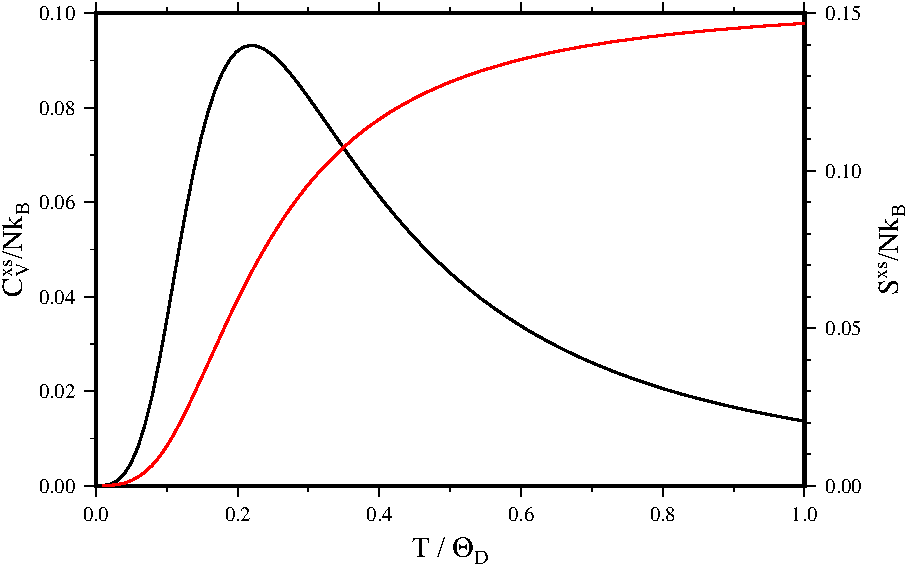
\includegraphics[width=0.8\textwidth]{figures/debye_excesses}
  \caption{Excess thermal properties as a function of temperature normalised to the Debye temperature, plotted for a reduction of 5\% in the Debye temperature.}
  \label{fig:debye_excesses}
\end{figure}


\subsection{Modelling excess properties}

\subsubsection{Fitting parameters}
When excesses are zero, the ideal model should be recovered, which (for a binary $A-B$) has the following properties:
\begin{eqnarray}
\mathcal{V}_{id} =& x_A\mathcal{V}_A + x_B\mathcal{V}_B,\label{eqn:ideal_volume} \\
\frac{\mathcal{V}_{id}}{K_{T, id}} =& x_A\frac{\mathcal{V}_{A}}{K_{T, A}} + x_B\frac{\mathcal{V}_{B}}{K_{T, B}}, \\
\alpha_{id} \mathcal{V}_{id} =& x_A\alpha_A \mathcal{V}_A + x_B\alpha_B \mathcal{V}_B 
\end{eqnarray}

Based on the observations reviewed in Section \ref{sec:obs}, two parameters are introduced, which describe the excess thermoelastic properties at the standard state volume:
\begin{eqnarray}
K_T =& K_{T, id} \left(\frac{V_{id}}{V}\right)^{\xi} \label{eqn:KV_relation} \\
\alpha K_T |_{V} =& \zeta \alpha_{id} K_{T, id} |_{V_{id}}
\end{eqnarray}
\noindent The parameter $\xi$ describes how quickly the excess volumes decrease with increasing pressure, and $\zeta$ is a term describing, to first-order, differences in thermal pressure (and therefore excess thermal properties). A value of $\zeta$=1 is consistent with data for the halite-sylvite solid solution \citep{WVCJCB2004, WVCCJB2005}, and other solutions should have values of $\zeta$ very close to unity. Figure \ref{fig:ksi} illustrates the range of $\xi$ for some liquid and solid solutions. Solutions with stronger interactions (ordering or complexation) tend to exhibit higher values of $\xi$, although a value of 7 provides a good approximation for many solutions. 

\begin{figure}[ht!]
  \centering
  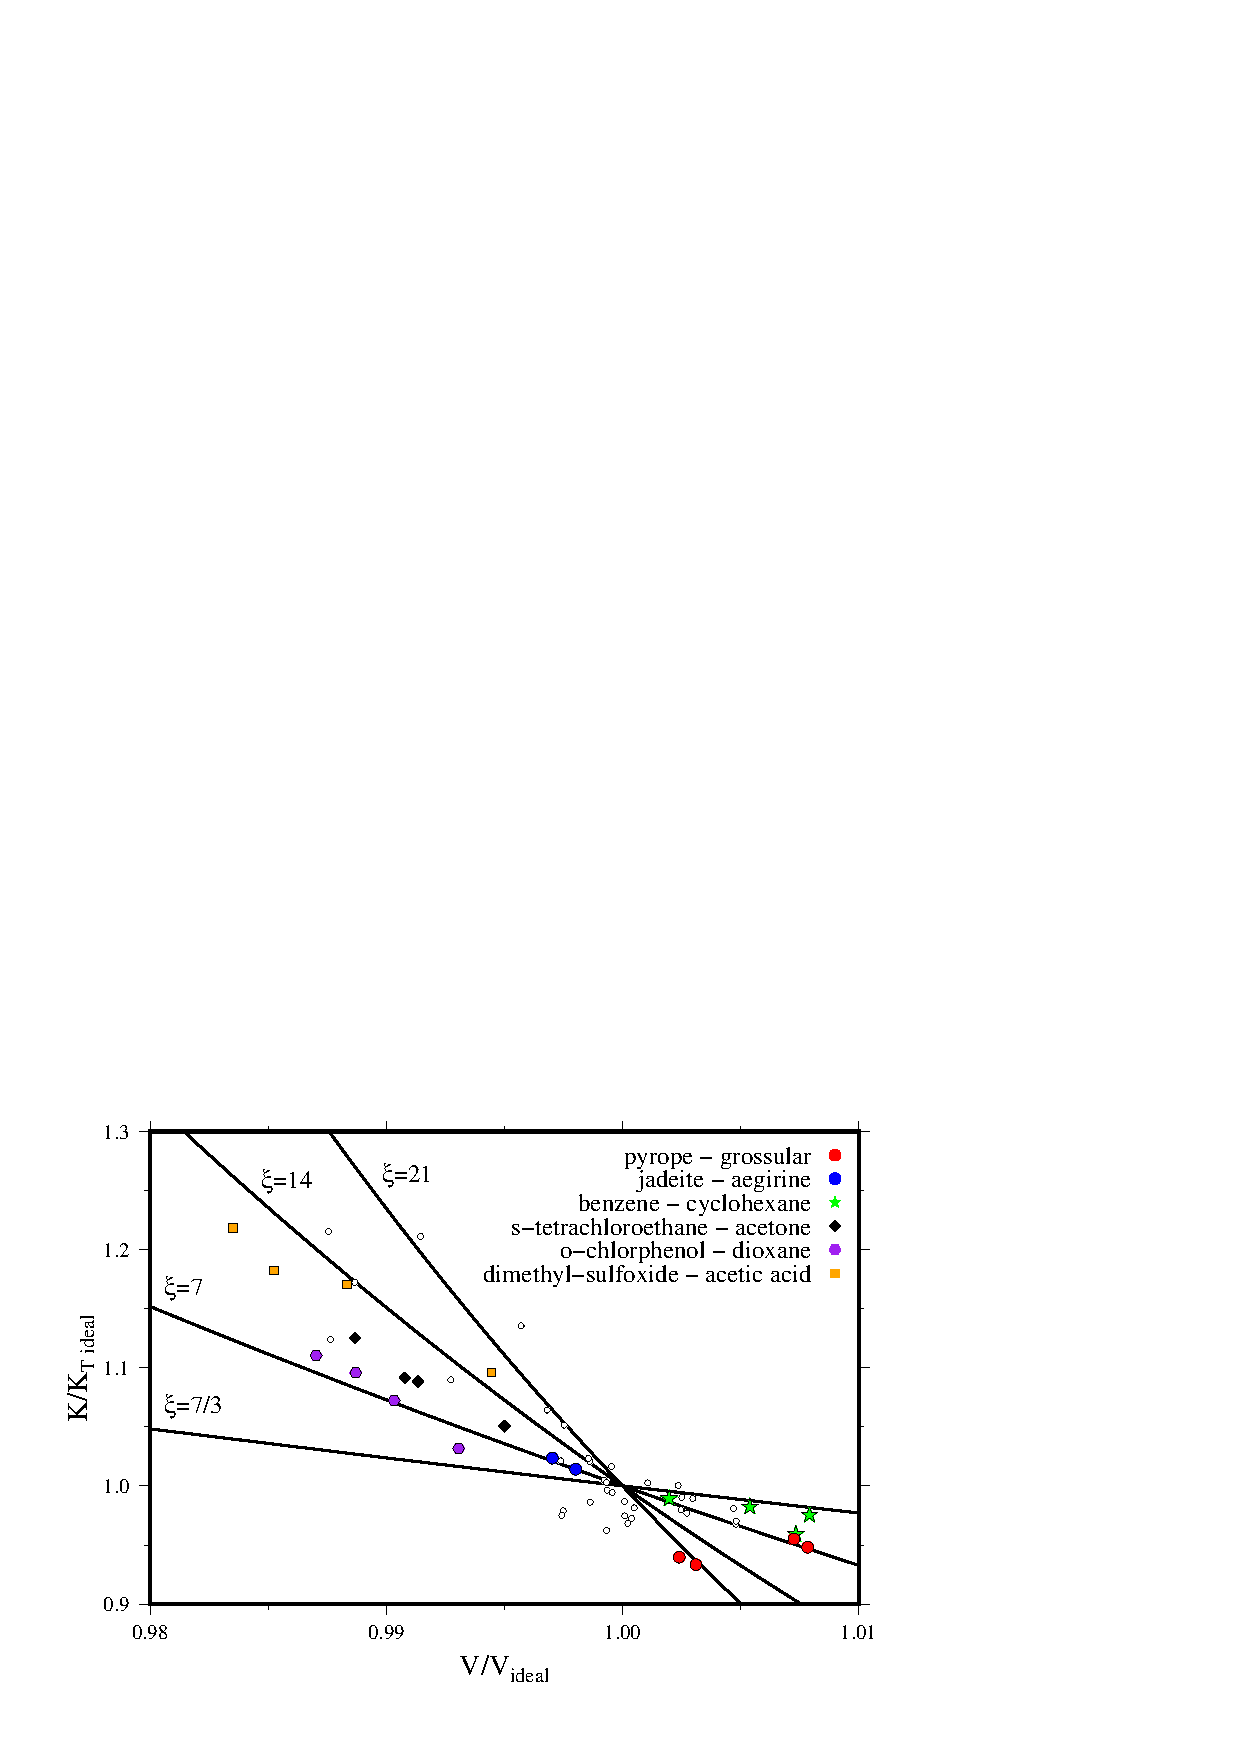
\includegraphics[width=0.8\textwidth]{figures/VK_ratio}
  \caption{Dependence of excess bulk moduli on excess volumes for a range of solid and liquid solutions. Pyrope-grossular \citep{DCW2015} and jadeite-aegirine data \citep{NBLBT2006} are plotted using the isothermal bulk modulus $K_T$, while the liquid data \citep{FM1965} uses the isentropic bulk modulus $K_S = K_T \left ( 1+ \gamma \alpha T \right)$. White symbols show the data for all 14 solutions studied by \cite{FM1965}.}
  \label{fig:ksi}
\end{figure}

Note that different compositions within the same solution often fall within a linear array in Figure \ref{fig:ksi}, suggesting that the use of a single value of $\xi$ may be justified for the entire compositional range of a binary solution. One notable exception is the pyrope-grossular data of \cite{DCW2015}, for which two compositions close to the endmembers displayed remarkably low bulk moduli (and therefore extremely high apparent values of $\xi$). The authors of this study did note a large degree of microstrain in these samples, which may not be representative of most geological materials. All of the solution data plotted in Figure \ref{fig:ksi} are best fit by values of $\xi > 7/3$, the value which would be required if any composition within a non-ideal solution were to be described by a second order Birch-Murnaghan equation of state. The implication is that an accurate description of excess volumes within solid solutions generally requires modifications to the constitutive endmember equations of state.


\subsubsection{An excess equation of state}
\label{sec:eos}

To use these two parameters, an excess property equation of state must be formulated. We start with the two-parameter Murnaghan equation of state:
\begin{equation}
  \frac{\mathcal{V}_P}{\mathcal{V}_0} = \left( 1 + \frac{K'_0 P}{K_0} \right)^{-1/K'_0}
\label{eqn:murn}
\end{equation}
\noindent where $P_{th}$ is the thermal pressure. In this study, it is assumed that excess volumes and excess vibrational entropies approach zero as $P \rightarrow \infty$. Applying Equation \ref{eqn:murn} to the ideal and nonideal compounds, and equating $V_P$ and $P$ at high pressure, we obtain the following equality:
\begin{equation}
\mathcal{V}_{0, id} \left( \frac{K'_{0, id}}{K_{0, id}} \right)^{-1/K'_{0, id}} = \mathcal{V}_{0} \left( \frac{K'_{0}}{K_{0}} \right)^{-1/K'_0}
\end{equation}
If the ideal and nonideal structures have the same $K'_0$, then Equation \ref{eqn:KV_relation} is satisfied, and we can substitute $K'_0$ with the parameter $\xi$. We now have a description of the excess volume as a function of pressure:
\begin{equation}
\mathcal{V}^{xs} = \mathcal{V}_0 \left(1 + \frac{\xi P}{K_0}\right)^{-1/\xi} - \mathcal{V}_{0, id} \left(1 + \frac{\xi P }{K_{0, id}}\right)^{-1/\xi} 
\end{equation}
\noindent As this expression only describes the excess volume, and does not affect the ideal volume, it is not necessary for $\xi$ to equal $K'_{0, id}$. In relaxing this constraint, we no longer require the total thermodynamic properties of the non-ideal phase to be governed by the Murnaghan equation of state. This freedom allows the excess equation of state to be used regardless of the equation of state of the endmembers. 

To calculate excess Gibbs Free energies at some pressure $P_1$ and temperature $T_1$, we take the pressure integral of the excess volumes along the isothermal path $T = T_0$ to infinite pressure, and the integral along $T = T_1$ from infinite pressure to $P_1$. The isobaric path from $T_0$ to $T_1$ at infinite pressure does not contribute to the excess free energy, as we assume that $S^{xs} = 0$ at infinite pressure. To calculate $G^{xs}$ along the high temperature path, we assume that the form of the excess volume curve is temperature-independent (i.e., that the excess bulk modulus and $\xi$ do not vary along the $V_0$ isochore). The heuristic parameter $\zeta$ provides an equation of state-independent method to calculate the thermal pressure. The excess energy is thus calculated from the following expressions

\begin{eqnarray}
\mathcal{G}^{xs} =& \int_{P_0}^\infty \mathcal{V} \, dP' |_{T0} - \int_{P_\textrm{eff}}^\infty \mathcal{V} \, dP' |_{T_1} ,\\
\int_{P}^\infty \mathcal{V}^{xs} \, dP' =& - \frac{\left(K_0 \mathcal{V}_0 \left(1 + \frac{\xi P}{K_0}\right)^{1-1/\xi} - K_{V0, T0, id} \mathcal{V}_{T, id} \left(1 + \frac{\xi P}{K_{V0, T0, id}}\right)^{1-1/\xi} \right) }{1 - \xi} ,\\
P_{\textrm{eff}} =& P_1 - P_{th} - P_0, \\
P_{th} =& \zeta P_{th, id} = \zeta \int_{T_0}^{T_1} \alpha_{id} K_{T, id} dT' 
\end{eqnarray}
\noindent $K_0$ for the non-ideal compound is calculated according to Equation \ref{eqn:KV_relation}. In practice, $P_{th, id}$ can be calculated by iteratively solving for the pressure at temperature $T$ where the ideal volume is the same as the standard ideal volume (Equation \ref{eqn:ideal_volume}). This algorithm can then be used regardless of the equation of state for the individual endmembers. Excess thermodynamic properties can now be calculated at any pressure and temperature by appropriate differentiation of $G^{xs}$. Figure \ref{fig:xs_model} shows the excess volumes and entropies predicted for the pyrope-grossular join using the current model.
\begin{figure}[ht!]
  \centering
  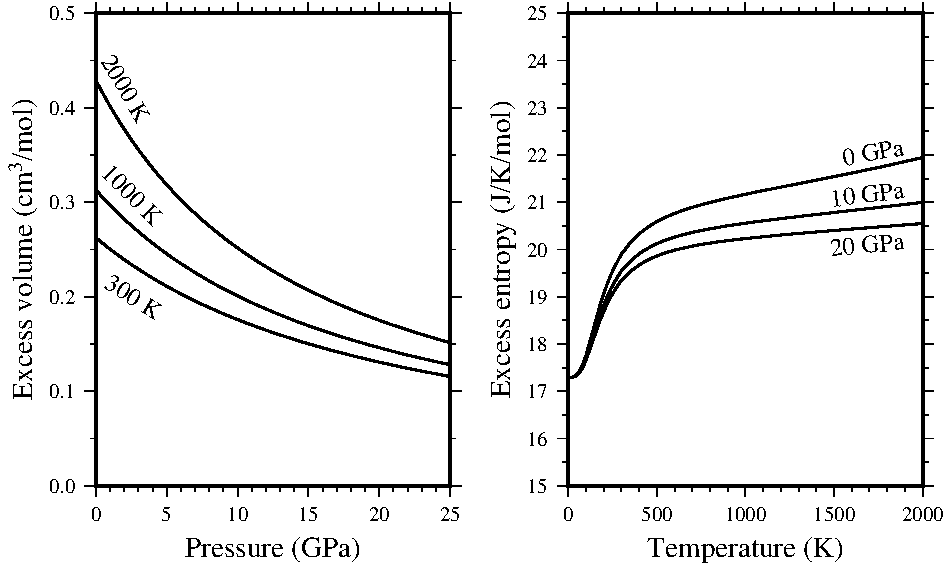
\includegraphics[width=0.8\textwidth]{figures/VSxs_pygr}
  \caption{Pyrope-grossular excesses for an excess volume at 1 bar, 300 K of 0.25 cm$^3$/mol, $\xi=7$ and $\zeta=1.005$. Note the similarities in the form of the excess entropy to that shown in Figure \ref{fig:debye_excesses}.}
  \label{fig:xs_model}
\end{figure}

%A useful way to view the change in bulk modulus across a solid solution is to compare the excess bulk modulus to that implied by the $K_TV =$ \emph{constant} rule of thumb proposed by \cite{AA1970} to estimate the compressibility of endmembers based on their molar volumes. The heuristic we propose in this study predicts a larger excess term than that suggested by the rule of thumb, which we describe using a factor $\xi$:

%\begin{equation}
% K_{T} \sim 0.5(K_{Ti} + K_{Tj}) + \xi \left(\frac{K_{Ti}\mathcal{V}_{j} + K_{Tj}\mathcal{V}_{j}}{2 \mathcal{V}} - 0.5(K_{Ti} + K_{Tj})\right)
%  \label{K_T_heuristic}
%\end{equation}
%\noindent Typically, a value of $\sim$6 provides a useful estimate of $\xi$.


%In the absence of any solid solution data, \cite{BD2011,BD2012} propose using the following equation to estimate excess heat capacities:
%\begin{eqnarray}
%\mathcal{S}^{xs, max} = a \Delta \mathcal{V} + b n \Delta K_T, \\
%\Delta \mathcal{V} = | V_{1} - V_{2} |, \\
%\Delta K_T = \frac{V_{1} - V_{2}}{| V_{1} - V_{2} |} \left( K_{T1} - K_{T2} \right)
%\end{eqnarray}
%\noindent where $n$ is the moles of ions involved in the exchange per mole of material and a and b are constants fit to experimental data. Fits to silicates, oxides and metal solutions yield values of 2.926e5 J/K/m$^3$ and 7.20e-11 J/K/Pa/mol \citep{BD2011} or 2.505e5 J/K/m$^3$ and 2.73e-11 J/K/Pa/mol \citep{BD2012}. The hypothesis underlying such equations is similar to that in the preceding section; inflated structures lead to lower frequency lattice vibrations and therefore higher heat capacities. However, the dependence on bulk modulus depends on the assumption that different cation-anion bonds have an intrinsic bond strength, which controls the magnitude and sign of the volume excess due to ion size mismatch. At least in metallic systems, bond strength is highly dependent on chemical environment \citep{WC2000}. For this reason, a simple linear dependence on bulk modulus is unlikely to be a good predictor of excess properties, which may explain the large difference in estimates for $b$.

% Estimated vibrational entropies of disordering in metal alloys may be as great as $0.5R$ \citep{TB1989; WC2002}, and therefore comparable with fully disordered configurational entropies ($\sqrt 2 R$). An increase in excess entropy with temperature must introduce an increase in the excess enthalpy, via the relation $\partial H / \partial T = T \partial S / \partial T$.

% Studies of the properties of the NaCl-KCl solid solution are in good agreement with the observations and hypotheses presented here. Excess heat capacities are positive at low temperature, and excess vibrational entropies are therefore also positive and on the order of 2 J/K/mol in the center of the binary \citep{BD2013}. Excess volumes, compressibilities and thermal expansivities are also generally positive, although sombrero-shaped excesses are reported across the solid solution for the high pressure thermal expansivities of \citep{WVCJCB2004, WVCCJB2005}.

\subsubsection{Formulation for solutions using the subregular (Margules) mixing model}

The subregular Margules mixing model within a binary system $A$-$B$ approximates excess Gibbs free energies at any given pressure and temperature as a cubic function of composition \citep{HW1989}:
\begin{equation}
  \mathcal{G}^{xs} = X_B (1-X_B) \left(W^{\mathcal{G}}_{AB} X_B + W^{\mathcal{G}}_{BA} (1-X_B) \right)
  \label{eqn:subreg}
\end{equation}

This form of solution model is frequently used in the geological literature, because even if it does not perfectly reproduce the form of the free energy of many solutions \citep{NW1980}, it often provides a good first order approximation and is trivially differentiable with respect to composition, yielding endmember activities which can then be used to efficiently calculate phase equilibria. In the special case that $W_{AB} = W_{BA}$, Equation \ref{eqn:subreg} reduces to a simple quadratic with a maximum excess free energy of 0.25$W_{AB}$. It is therefore reasonable to use the following expressions:
\begin{eqnarray}
W^{\mathcal{G}}_{AB} = 4 \mathcal{G}^{xs}_{AB},\\
W^{\mathcal{V}}_{AB} = 4 \mathcal{V}^{xs}_{AB}
\end{eqnarray}
\noindent where $G^{xs}_{AB}$ is derived from the model described in Section \ref{sec:eos}. For a symmetric solution, $G^{xs}_{AB}$ thus describes the excess Gibbs free energy of the compound $A_{0.5}B_{0.5}$.


Expanding the subregular solution model beyond a binary system, the excess nonconfigurational Gibbs free energy for a subregular solution model is \citep{HW1989} 
\begin{equation}
  \mathcal{G}^{xs} = \sum_{i=1}^n \sum_{j>1}^n X_i X_j \left ( W^{\mathcal{G}}_{ij} X_j + W^{\mathcal{G}}_{ji} X_i + 0.5 (W^{\mathcal{G}}_{ij} + W^{\mathcal{G}}_{ji}) \sum_k^n (1-\delta_{ik})(1-\delta_{jk}) X_k \right)
  \label{xs}
\end{equation}

\section{Examples}
Now that we have described the new model and heuristics related to the construction of intermediate compounds, we turn to a few geologically relevant examples. The models in this study are all implemented in the open software \emph{burnman}, a mineral physics toolkit written in python. The software, first described in \cite{CHRU2014}, was originally designed for seismic velocity calculations. It has since been augmented with thermodynamics functionality, including a range of different models for solid solutions.


\subsection{Pyroxene}
The first example is that of jadeite-aegirine pyroxene, a solid solution which displays a small volumetric deviation from ideality. The experimental data is that of \cite{NBLBT2006}. The Modified Tait equation of state \citep{HP2011} is used for the endmembers. The fit to the volume data is shown in Figure \ref{fig:PV_jadeite_aegirine}.

\begin{figure}[ht!]
  \centering
  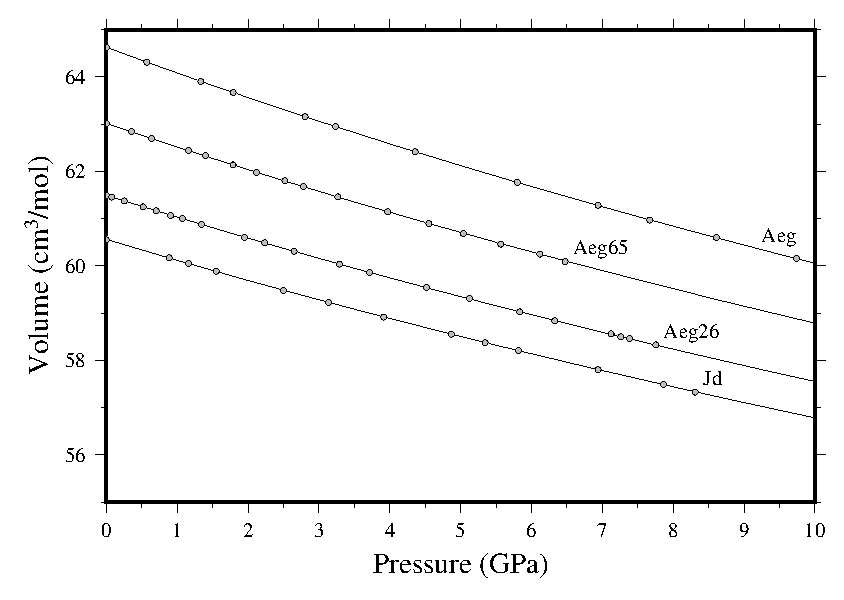
\includegraphics[width=0.8\textwidth]{figures/jadeite_aegirine_P_V}
  \caption{Pressure-volume data in the binary system jadeite-aegirine \citep{NBLBT2006}. Solid lines correspond to the volumes predicted by the model proposed in this study.}
  \label{fig:PV_jadeite_aegirine}
\end{figure}

\begin{table}[ht!]
\centering
\caption{Jadeite-Aegirine mixing parameters to fit the room temperature data of \cite{NBLBT2006}. *Additional constraint: $\xi_{ij} = \xi_{ji}$.}
\label{tab:jd_aeg}
\begin{tabular}{lllll}
                                               & jadeite                        & aegirine                     & $W_{\textrm{jdae}}$                  & $W_{\textrm{aejd}}$             \\
$\mathcal{V}_0$, $\mathcal{V}^{xs}$ (cm$^3$/mol) & 60.562 $\pm$ 0.002 & 64.628 $\pm$ 0.004 & -0.98 $\pm$ 0.02    & -0.52 $\pm$ 0.02 \\
$K_0$, $\xi$ (GPa)                   & 133.8 $\pm$ 0.2       & 116.0 $\pm$ 0.2       & 5.27  $\pm$ 0.74    & 5.27 $\pm$ 0.74*      \\
$K'_0$             & 4.6 [fixed]                 & 4.4 [fixed]                 &              & 
\end{tabular}
\end{table}

Using the derived properties of the solid solution, we can fit the excess volume as a function of pressure (Figure \ref{fig:excess_volume_jadeite_aegirine}). The decay of excess volume as a function of pressure is in excellent agreement with the assumption that excess volumes decay to zero at extreme pressures. Individually, the excess volumes for the two intermediate solutions are best fit by a value of $\xi = 7$ (Equation \ref{eqn:KV_relation}), which is somewhat lower than the value of 5.3 $\pm$ 0.7 obtained from simultaneous fitting of the equations of state. However, given the uncertainty in the volume data, the difference in values is negligible.

\begin{figure}[ht!]
  \centering
  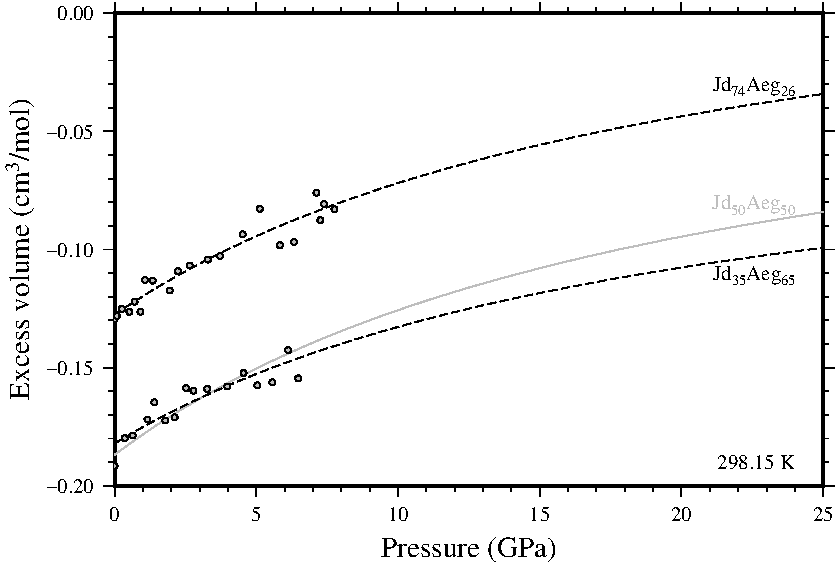
\includegraphics[width=0.8\textwidth]{figures/jadeite_aegirine_Vex}
  \caption{Excess volume for jadeite-aegirine pyroxenes \citep{NBLBT2006}. Solid lines correspond to the modelled excess volumes.}
  \label{fig:excess_volume_jadeite_aegirine}
\end{figure}

\subsection{Garnet}
Our first example dealt with a solid solution which has small excess volumes, but some phases exhibit significantly larger excesses. One example is the garnet system. Of particular interest is the pyrope-grossular join. Grossular is a major secondary component of many natural pyropic garnets. The size mismatch between the small magnesium cation and the large calcium cation on the dodecahedral site results in a large positive excess volume \citep{NCK1977, BG1997, GCT1996}. Recently, it has been suggested that the excess volumes of mixing are $\sim$1 cm$^3$/mol, 2--3 times larger than previously considered, and associated with very large negative excess bulk moduli \citep{DCW2015}. It is proposed that the differences are due to a hydrogrossular component in the crystals synthesised in piston cylinder apparatus in earlier studies, which becomes unstable at high pressures. Such a large variation in bulk modulus would have a major impact on seismic velocities and excess properties at high pressure. Since garnets remain stable to the uppermost lower mantle, a careful analysis of these effects is warranted.

Here, we create four models to describe the room temperature equations of state for the pyrope-grossular system using the pyrope and grossular endmembers from \cite{HP2011}. Two models are presented for the data of \citep{DCW2015}, to describe the reported behaviour close to the center and at the edges of the solid solution. The third model is the constant volume subregular Margules model of \cite{GCT1996}. A fourth model has the same excess volume as \cite{GCT1996}, but a negative excess bulk modulus which allows the excess volume to decay to zero at high pressures ($\xi=6$). The standard state bulk moduli are shown in Figure \ref{fig:K_T_pyrope_grossular}.


\begin{figure}[ht!]
  \centering
  %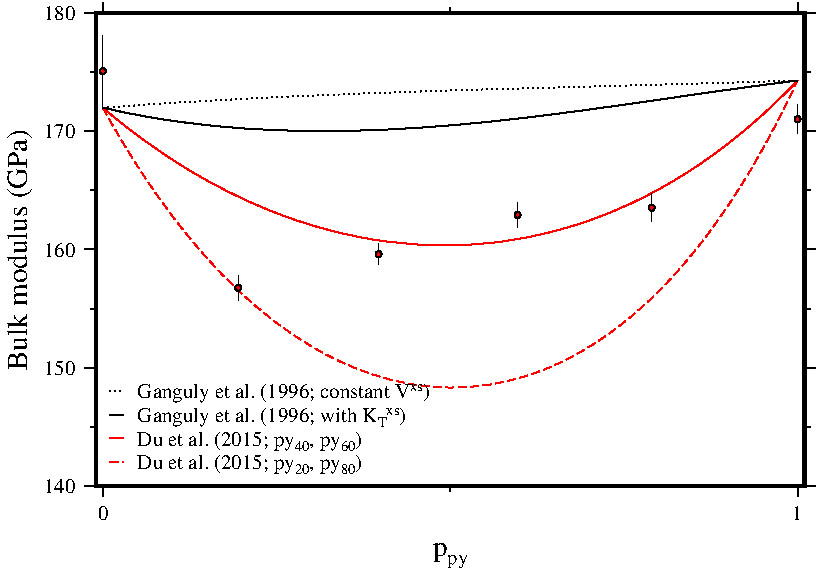
\includegraphics[width=0.8\textwidth]{figures/pyrope_grossular_K_0}
  \caption{Bulk moduli in the pyrope-grossular binary. Data points are those reported by \cite{DCW2015}. The four models correspond to those discussed in the main text.}
  \label{fig:K_T_pyrope_grossular}
\end{figure}

It is immediately obvious that the bulk moduli calculated from the \cite{DCW2015} study exhibit very large deviations from a linear trend. The symmetric curve derived from the two compounds in the middle of the binary yields $\xi=10$, a value which is not unreasonable, and results in a change in sign of the volume excess at 20--25 GPa. In contrast, the trend derived from the compounds with 20\% and 80\% pyrope content yields $\xi=52$. This extreme value leads to negative excess volumes at 5--6 GPa, which does not seem to be very likely. To avoid this, $K'_T$ must be increased to $>$20, which is also extremely unlikely.

The trend calculated from the terms in \cite{GCT1996} has a small positive excess bulk modulus, which is always the case where $\mathcal{V}^{xs}$ is held fixed. For the reasons outlined in the introduction, this is probably unlikely. The final model, constructed using the heuristics described in the previous section yields an excess bulk modulus on the order of 2--3 GPa.

These models are now used to illustrate the effect of different excess volume models on seismic wave velocities. P-wave, S-wave and bulk sound velocities are functions of isentropic bulk and shear moduli and density:
\begin{eqnarray}
V_P = \sqrt \frac{K_S + \frac{4}{3} G }{\rho} \\
V_S = \sqrt \frac{G}{\rho} \\
V_\Phi = \sqrt \frac{K_S}{\rho}
\end{eqnarray}
Thermodynamic solution models say nothing about shear moduli, so we restrict our discussion to the bulk sound velocity. Figure \ref{fig:bulk_sound_garnet} shows the bulk sound velocity at ambient temperature for the four solid solution models in the text. The models of \cite{DCW2015} result in large depressions of bulk sound velocity. The model constructed from the py$_{40}$ and py$_{60}$ samples results in a 4\% depression relative to the constant $\mathcal{V}^{xs}$ case throughout the upper mantle pressure range. In contrast, the model based on the excess volume model proposed in \cite{GCT1996} predicts a 1\% decrease in bulk sound speed. 

\begin{figure}[ht!]
  \centering
  %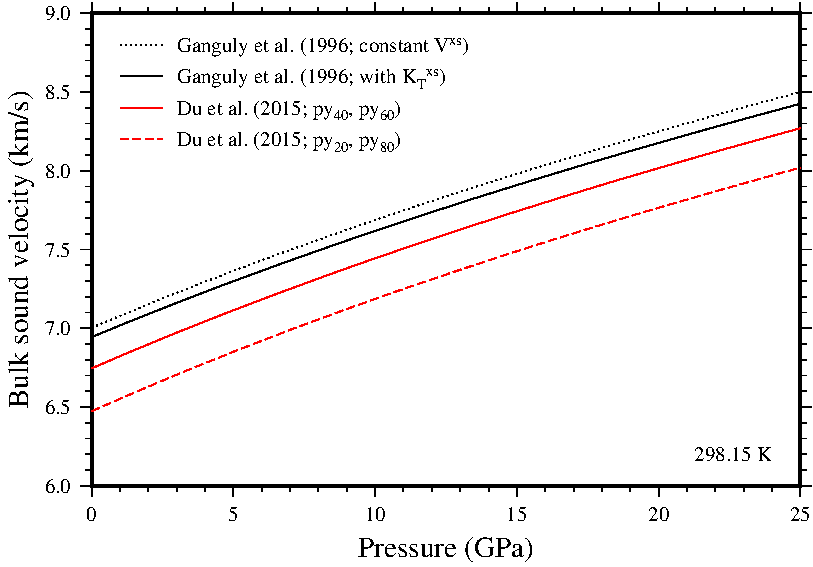
\includegraphics[width=0.8\textwidth]{figures/pyrope_grossular_bulk_sound_velocities}
  \caption{Bulk sound velocities of py$_{50}$gr$_{50}$ at room temperature according to the models described in the text and in Figure \ref{fig:K_T_pyrope_grossular}.}
  \label{fig:bulk_sound_garnet}
\end{figure}

It is not yet clear whether natural garnets have P-V-T equations of state similar to those suggested by \cite{DCW2015}, or similar to those in previous studies \citep{NCK1977, BG1997, GCT1996}. If a hydrogrossular component is indeed the cause for low excess volumes in piston cylinder-synthesised garnets, then garnets in the mantle are likely to have relatively high volume excesses and low bulk moduli. In this case, constant V$^{xs}$ models are clearly inappropriate both for calculations of mantle phase relations and seismic velocities. Even in the case of the model derived from \cite{GCT1996}, the difference in free energy compared with the constant V$^{xs}$ model is on the order of kilojoules at the bottom of the mantle transition zone. 

The heuristics suggested here place constraints on seismic properties which are significantly more strict than typical uncertainties on bulk moduli derived from ultrasonic interferometry, Brillouin scattering or static compression. For example, along the pyrope-majorite join, excess volumes are small (0.1 cm$^3$/mol) \citep{HSSR1997}. With the assumption that excess volumes decrease to zero with increasing pressure, the excess bulk modulus is constrained to be $\sim$-0.6 GPa. In comparison, the range in bulk modulus estimates anywhere along the pyrope-majorite join is about 10 GPa \citep[see, for example][]{HDLWB2010}. So far, high pressure elasticity studies have mostly been focussed on binary joins with small excess volumes at ambient pressure \citep{FXMLX2015, HC2014}. That they should exhibit small excess bulk moduli is in excellent agreement with the heuristics proposed here, but a far more rigorous test would be to investigate systems with large volume excesses.

\subsection{Metallic-ionic melt}
The thermodynamics and thermoelastics of ionic and metallic melts is fundamental to our understanding of core differentiation. During the formation of the terrestrial planets, it is thought that oligarchic growth led to a series of mixed silicate-metallic magma oceans, from which metallic melts separated before sinking as diapirs into the growing core \citep{Rubieetal2015}. Although these melts are predominantly composed of iron and nickel, several weight percent of light elements are required to explain the Earth's density deficit and low seismic velocities \citep{Poirier1994}. These light elements not only influence the melting point of the core (which directly informs us about the temperature of the inner core boundary), but also the style of crystallisation, and therefore the generation of a magnetic dynamo \citep{SSWL2007}. Since equilibration with a magma ocean governs the initial composition of the core, and seismology presents us with the most direct information on the present composition of the core, accurate thermodynamic modelling is vitally important to our understanding of the evolution and present chemical state of the Earth. It is well known that several iron-light element binaries are associated with large non-idealities \citep[e.g.][]{Frostetal2010}, so accurate modelling requires changes in excess properties in these systems to be taken into account.

Oxygen is a good example of a light element which exhibits a large degree of non-ideality. At pressures $<$25 GPa, the Fe-FeO solution exhibits significant non-ideality, with a large miscibility gap between ionic and metallic Fe-O liquids \citep{KS1995,TOT2007,Frostetal2010}. As pressure increases, this miscibility gap disappears, indicating a negative excess volume of mixing (Figure \ref{fig:Fe_O_solvus}).

\begin{figure}[ht!]
  \centering
  %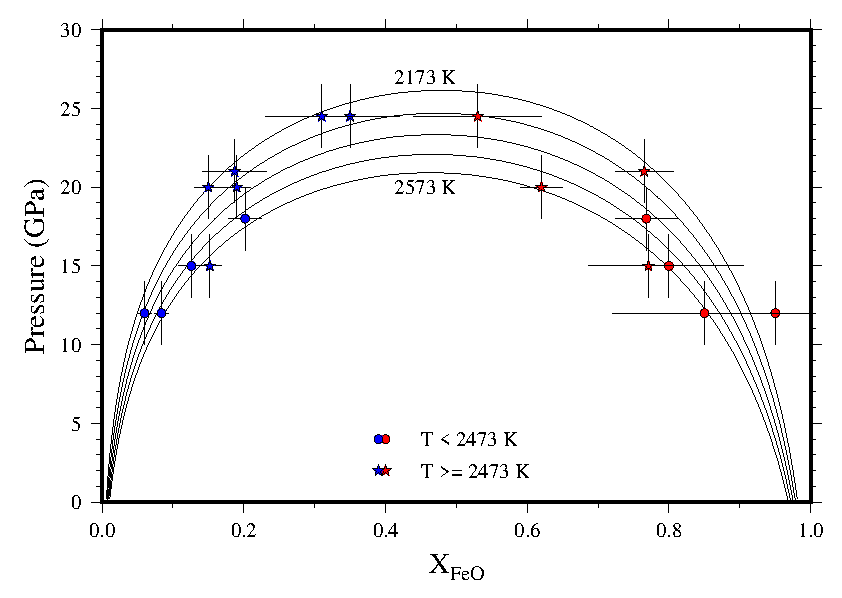
\includegraphics[width=0.8\textwidth]{figures/Fe_FeO_solvus}
  \caption{The Fe-FeO solvus as a function of pressure and temperature. Data points are taken from the studies of \cite{TOT2007} and \cite{Frostetal2010}. The model corresponds to the values proposed in Table \ref{tab:Fe_FeO}.}
  \label{fig:Fe_O_solvus}
\end{figure}

To constrain the properties of the Fe-FeO solid solution, the chemical potentials of Fe and FeO are estimated from the compositions of coexisting ionic and metallic melts at $<$25 GPa, and the pressure, temperature and compositions of eutectic liquid at $>$25 GPa \citep{SHCPW2008}. The latter constraints also require thermodynamic data for the eutectic phases (B1-structured FeO and FCC and HCP iron), which are calculated from room pressure data and constraints on the melting curves \citep{SHCPW2008, OTHOH2011, ADMLM2013, Kom2014}.  The Margules parameters estimated from this data are shown in Figure \ref{fig:Fe_O_interaction}. 

\begin{figure}[ht!]
  \centering
  %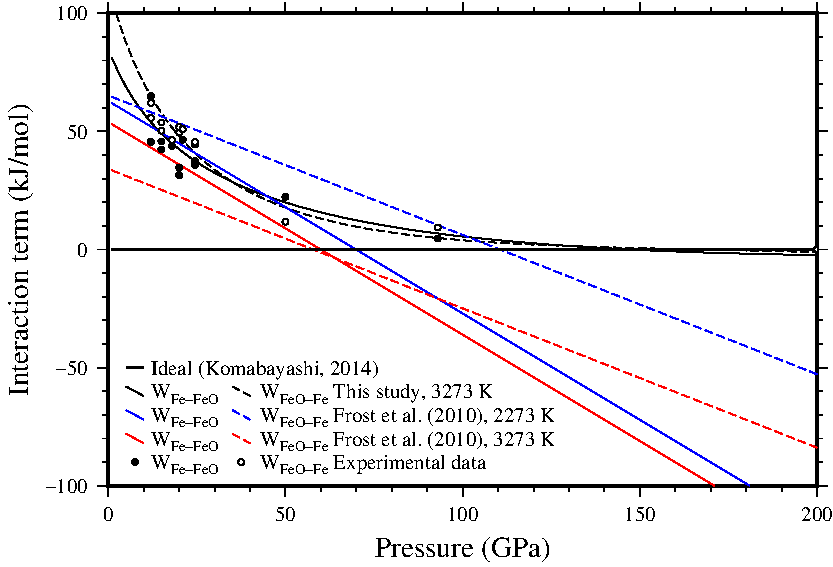
\includegraphics[width=0.8\textwidth]{figures/Fe_FeO_interaction_terms}
  \caption{Interaction terms in Fe-FeO melt as a function of pressure. Experimental data comes from solvus constraints at $<$25 GPa \citep{TOT2007,Frostetal2010}, and the composition and temperature of the eutectic at higher pressures \citep{SHCPW2008}.}
  \label{fig:Fe_O_interaction}
\end{figure}

The uncertainties on composition and temperature of the eutectic are rather large, so these data are supplemented by the requirement that excess volumes become zero at very high pressure. The parameters used to create the fits in Figures \ref{fig:Fe_O_interaction} and \ref{fig:Fe_O_melting} are given in Table \ref{tab:Fe_FeO}. It is assumed that excess entropy and thermal expansion are negligible. The majority of the $<$25 GPa data was collected within a $\sim$200 K temperature range, and is associated with similar temperature uncertainties, which introduces very large uncertainties in excess entropies. Add to that the possibility of phase separation during quench and the large uncertainty in coexisting ionic/metallic melt compositions, there is no clear evidence for the large temperature dependence proposed by \cite{Frostetal2010}, although they do slightly improve the fit to the data (mostly by increasing the pressure at which the solvus closes at high temperature).

\begin{figure}[ht!]
  \centering
  %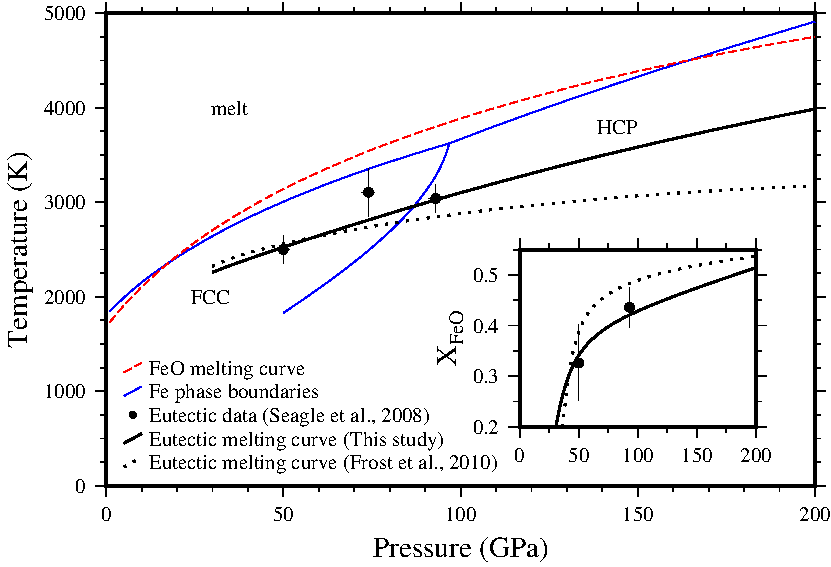
\includegraphics[width=0.8\textwidth]{figures/Fe_FeO_T_X_eutectic}
  \caption{Melting temperature in the Fe-O system as a function of pressure. Inset: eutectic composition in the Fe-O system. Data points are from \cite{SHCPW2008}. The model of \cite{Frostetal2010} employs constant volume and entropy terms derived from data obtained at $<$25 GPa, and deviates significantly from experimental constraints at pressures corresponding to the Earth's core.}
  \label{fig:Fe_O_melting}
\end{figure}

\begin{table}[ht!]
\centering
\caption{Excess Fe-FeO mixing parameters to fit the data in Figures \ref{fig:Fe_O_interaction} and \ref{fig:Fe_O_melting} at a reference temperature of 1809 K and pressure of 50 GPa.}
\label{tab:Fe_FeO}
\begin{tabular}{lll}
  Property        & Fe$_{50}$FeO$_{50}$  & FeO$_{50}$Fe$_{50}$ \\
  $H^{xs}$ (J/mol) &  5000 $\pm$ 400 & 4400 $\pm$ 400  \\
  $S^{xs}$ (J/K/mol)  & 0 [fixed] & 0 [fixed] \\
  $V^{xs}$ (cm$^3$/mol)   & -0.117 $\pm$ 0.009 &  -0.138 $\pm$ 0.009 \\
  $K^{xs}$  (GPa)  & 28 $\pm$ 5 & 45 $\pm$ 5  \\
  $K'^{xs}$   & -0.07 $\pm$ 0.12 & -0.37 $\pm$ 0.12  \\
  $a^{xs}$   & 0 [fixed] & 0 [fixed]  
\end{tabular}
\end{table}


The constant negative volume excesses in the model of \cite{Frostetal2010} produce reasonable eutectic melting temperatures up to $\sim$ 50 GPa. Beyond this point, the increasing pressure stabilisation of the solution results in large deviations from the slope of the melting curve (Figure \ref{fig:Fe_O_melting}). This effect becomes very large at inner core boundary pressures (330 GPa), where solid Fe and FeO coexist to at least $\sim$4200 K \citep{OTHOH2011}. In contrast, the melting curve derived from the parameters of \cite{Frostetal2010} reaches a maximum at 3225 K and 275 GPa. The best fit excess bulk moduli in Table \ref{tab:Fe_FeO} are large, even at the reference pressure of 50 GPa. Such values will have a significant effect on seismic velocities, especially at the pressures corresponding to the cores of small planetary bodies.


\section{Discussion}
% Intro
The use of intermediate compounds to describe excess properties within the framework of simple solution models lends the flexibility required to create single thermoelastodynamic models covering very large \emph{P-T} ranges. In this study, the high pressure properties of pyroxenes, garnets and melts are used to illustrate the development of such models, and their ability to accurately reproduce observed variations in pressure, temperature or compositional derivatives of the Gibbs free energy, such as bulk modulus and chemical potentials. Without these, it would be impossible to accurately model phase relations at extreme conditions, or seismic velocities.

This study does not discuss the behaviour of the shear modulus across solid solutions. Thermodynamic databases are now starting to include shear moduli and their change with pressure and temperature \citep{SLB2011}, so constraining these changes across solid solutions should also be a key priority for experimental and ab-initio studies. Using intermediate compounds to describe the change in shear modulus across a solid solution should work well, especially in silicate systems, where excess shear moduli may be of similar magnitude to excess bulk moduli, and also decrease with increasing pressure \citep[e.g][]{LEDD2014}.

% Heuristics
The heuristics suggested in this study agree with the available data on the three example systems, but remain heuristics only. It would be particularly interesting to investigate the change in excess volumes with temperature and pressure for other systems in which excess properties are large, and interpret these in terms of crystal or melt structures. Conversely, the behaviour of systems with small excesses at room temperature and pressure should also be investigated. Current evidence suggests that small volume excesses at low pressure remain small under different conditions \citep{FXMLX2015, HC2014}, but this may not be true for all solutions.

% Other planets
In the case of ionic and metallic melts, excess volumes can be extremely large at low pressure. The large excess elastic moduli accompanying these excess volumes will have a large effect on seismic velocities, especially in the cores of relatively small bodies such as Mars or the Moon. As pressures increase, excess volumes are much reduced, which has a similarly profound effect on thermodynamic properties \citep{Frostetal2010, DKS2013}. Accurate characterisation of excess properties of melt solutions, and indeed of solutions in general, will become increasingly important for our interpretation of seismic anomalies, modelling of phase relations, and our understanding of planetary evolution. 

% Williams et al. 2015
\citep{WMSF2015}

\begin{acknowledgements}
The author is funded by the Advanced ERC Grant awarded to the ``ACCRETE'' project (Contract number 290568). He would like to thank Dave Rubie, Dan Frost and Christopher Beyer for useful discussions.

Figures were created using the Generic Mapping Tools \citep{GMT}.
\end{acknowledgements}

\bibliographystyle{spbasic}
\bibliography{references_xs}


\end{document}

\grid
